\documentclass[11pt,a4paper]{article}
\usepackage[utf8]{inputenc}
\usepackage{amsmath}
\usepackage{amsfonts}
\usepackage{amssymb}
\usepackage[pdftex]{graphicx}
\setlength{\parindent}{0in}
\begin{document}
\tableofcontents
\newpage

\section{Vision}
\subsection{Introduction}
Our goal is to make an interactive document sharing system, Slice of Pie,  which allows multiple users to share and edit documents both online and offline.
\subsection{Problem statement}
Sharing and editing documents can be cumbersome. \\
Sending a document back and forth between multiple users can lead to a lot of errors. Users can overwrite what another user has done, and if they aren't all using the same text editing system this can lead to formatting issues in the document.
\subsection{Summary of system features}
\begin{enumerate}
\item Multiple users must be able to share and edit documents online.
\item Synchronization for offline usage.
\item Merging of documents.
\item History. Which allows the user to see all recent changes made to the document.
\item Documents can be categorized into folders or projects in order to get a better overview when working on a larger project with multiple files.
\end{enumerate}

\section{Use cases}
\begin{enumerate}
\item UC1: Create new document
\item UC2: Edit document
\item UC3: Delete document
\item UC4: Merging documents (resolve conflict)
\item UC5: Offline sync
\item UC6: New folder
\item UC7: New project
\item UC8: Find old version of document
\end{enumerate}

% Use case 1
\fbox{\begin{minipage}{\columnwidth}
		\textbf{Use case UC1: Create new document} \\ 
		\textbf{Scope:} Slice-of-pie application \\
		\textbf{Level:} User goal \\
		\textbf{Primary actor:} Regular user \\
		\textbf{Stakeholders and Interests: } \\
		- Regular user: Wants to create a new document without any complications. \\
		\textbf{Preconditions:} none. \\
		\textbf{Postconditions:} The document must be created\\
		
		\textbf{Basic flow:} 
		\begin{enumerate}
			\item The user needs a document that can be shared with others.
			\item The user chooses a client program (web or desktop client).
			\item The user presses the "New Document" button.
			\item The client presents a dialogue box.
			\item The user types information about the document and press OK.
			\item The client sends a request to the server and the document gets stored by the server.
			\item The client displays the document for the user.
		\end{enumerate} 
		\textbf{Extensions:}
			\begin{enumerate}
				\item[6.]  The server is not responding \\
				\begin{enumerate}
					\item The document is saved locally.
					\item The client requests the server in regular intervals to see if it has recovered.
				\end{enumerate}
			\end{enumerate}
		\textbf{Special requirements:} \\
		- The document should be displayed properly on any devices such as smart phones and tablets. \\
\end{minipage}}

% Use case 2
\fbox{\begin{minipage}{\columnwidth}
		\textbf{Use case UC2: Edit document} \\ 
		\textbf{Scope:} Slice-of-pie application \\
		\textbf{Level:} User goal \\
		\textbf{Primary actor:} Regular user \\
		\textbf{Preconditions:} A document must have been created \\
		\textbf{Postconditions:} The document must be edited the way the user desires and the change must be recorded by the server too\\
		
		\textbf{Basic flow:} 
		\begin{enumerate}
			\item The user opens a document.
			\item The user edits the content of the document.
			\item The client sends a request to the server.
			\item The document is changed on the server.
		\end{enumerate} 
		\textbf{Extensions:}
			\begin{enumerate}
				\item[3.]  The server is not responding \\
				\begin{enumerate}
					\item The document is saved locally.
					\item The client requests the server in regular intervals to see if it has recovered.
				\end{enumerate}
			\end{enumerate}
		\textbf{Special requirements:} \\
		- The document should be displayed properly on any devices such as smart phones and tablets. \\		
\end{minipage}}

% Use case 3
\fbox{\begin{minipage}{\columnwidth}
		\textbf{Use case UC3: Delete document } \\ 
		\textbf{Scope:} Slice-of-pie application\\
		\textbf{Level:}  User goal\\
		\textbf{Primary actor:} Regular user\\
		\textbf{Preconditions:} A document must have been created. The user trying to delete a document must have sufficient rights to delete selected document\\
		\textbf{Postconditions:} The document is now deleted from the users local repository, and will be deleted when user commits\\
		
		\textbf{Basic flow:}
		\begin{enumerate}
			\item The user selects a document
			\item The user tries to delete the document
			\item The client sends a request to the server
			\item Server checks for authentication
			\item Document is deleted
		\end{enumerate}
		\textbf{Extensions:}
		\begin{enumerate}
			\item[3.] The server is not responding
			\begin{enumerate}
				\item The document is saved locally
				\item The client requests the server in regular intervals to see if it has recovered
			\end{enumerate}
			\item[4.] The user lacks the right to delete the selected document
			\begin{enumerate}
				\item User is told that he has not got the rights to delete selected document
			\end{enumerate}
		\end{enumerate}
		\textbf{Special requirements:} \\
\end{minipage}}	

% Use case 4
\fbox{\begin{minipage}{\columnwidth}
		\textbf{Use case UC4: Merging documents (Resolve conflict)} \\ 
		\textbf{Scope:} \\
		\textbf{Level:}  \\
		\textbf{Primary actor:} \\
		\textbf{Preconditions:} \\
		\textbf{Postconditions:} \\
		
		\textbf{Basic flow:} \\
		\textbf{Extensions:} \\
		\textbf{Special requirements:} \\
\end{minipage}}

% Use case 5
\fbox{\begin{minipage}{\columnwidth}
		\textbf{Use case UC5: Offline synchronization} \\ 
		\textbf{Scope:} Slice-of-pie application\\
		\textbf{Level:}  User goal\\
		\textbf{Primary actor:} Regular user\\
		\textbf{Preconditions:} User must be logged in. Client must be connected to the server\\
		\textbf{Postconditions:} The users offline repository will be synchronized with his online repository\\
		
		\textbf{Basic flow:} 
		\begin{enumerate}
			\item The user selects offline synchronization
			\item The client sends a request to the server
			\item The the server copies the user's online repository and sends it to the client
			\item The client sends verification upon receiving the documents 
		\end{enumerate}
		\textbf{Extensions:} 
		\begin{enumerate}
			\item[2.] The server is not responding
			\begin{enumerate}
				\item The user gets an error message (no connection)
			\end{enumerate}
			\item[3.] No connection between server and client
			\begin{enumerate}
				\item Request times out if server does not receive a verification form the client
				\item The user gets an error message (request timed out / no connection)
			\end{enumerate}
			\item[4.] The server is not responding
			\begin{enumerate}
				\item the client tries to reestablish a connection to the server at regular intervals, and then sends the verification
			\end{enumerate}
		\end{enumerate}
		\textbf{Special requirements:} \\
\end{minipage}}

% Use case 6
\fbox{\begin{minipage}{\columnwidth}
		\textbf{Use case UC6: Create new folder} \\ 
		\textbf{Scope:} \\
		\textbf{Level:}  \\
		\textbf{Primary actor:} \\
		\textbf{Preconditions:} \\
		\textbf{Postconditions:} \\
		
		\textbf{Basic flow:} \\
		\textbf{Extensions:} \\
		\textbf{Special requirements:} \\
\end{minipage}}

% Use case 7
\fbox{\begin{minipage}{\columnwidth}
		\textbf{Use case UC7: Create new project} \\ 
		\textbf{Scope:} \\
		\textbf{Level:}  \\
		\textbf{Primary actor:} \\
		\textbf{Preconditions:} \\
		\textbf{Postconditions:} \\
		
		\textbf{Basic flow:} \\
		\textbf{Extensions:} \\
		\textbf{Special requirements:} \\
\end{minipage}}

% Use case 8
\fbox{\begin{minipage}{\columnwidth}
		\textbf{Use case UC8: View old version of document} \\ 
		\textbf{Scope:} \\
		\textbf{Level:}  \\
		\textbf{Primary actor:} \\
		\textbf{Preconditions:} \\
		\textbf{Postconditions:} \\
		
		\textbf{Basic flow:} \\
		\textbf{Extensions:} \\
		\textbf{Special requirements:} \\
\end{minipage}}

\section{Glossary}

\section{Supplementary Specification (FURPS+)}
\begin{itemize}
\item Functionality
	\begin{itemize}
	\item The system must be able to store documents.
	\item The system must support multiple users.
	\end{itemize}
\item Usability
	\begin{itemize}
	\item The system must have a clean and simple user interface.
	\item Users must be able to use the application without training.
	\item System features must be simple and straight forward. No complicated work flows.
	\item The overall system must be easy to use. 8 out of 10 users must be able to use the system without any training.
	\end{itemize}
\item Reliability
	\begin{itemize}
	\item The system must be able to restore it's state in case of a server failure.
	\end{itemize}
\item Performance
	\begin{itemize}
	\item The system must be fast and responsive. A request to the system can't take longer than 3 seconds. (not counting the external internet connection)
	\end{itemize}
\item Supportability
\end{itemize}

\section{Domain Model}
	\begin{figure}[h!]
  		\centering
    	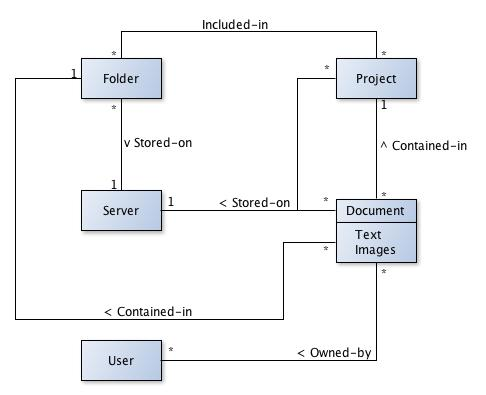
\includegraphics[width=300px]{images/DomainModel.jpg}
    	\caption{Domain Model}
	\end{figure}
	
\section{Logical Architecture}
	\begin{figure}[h!]
  		\centering
    	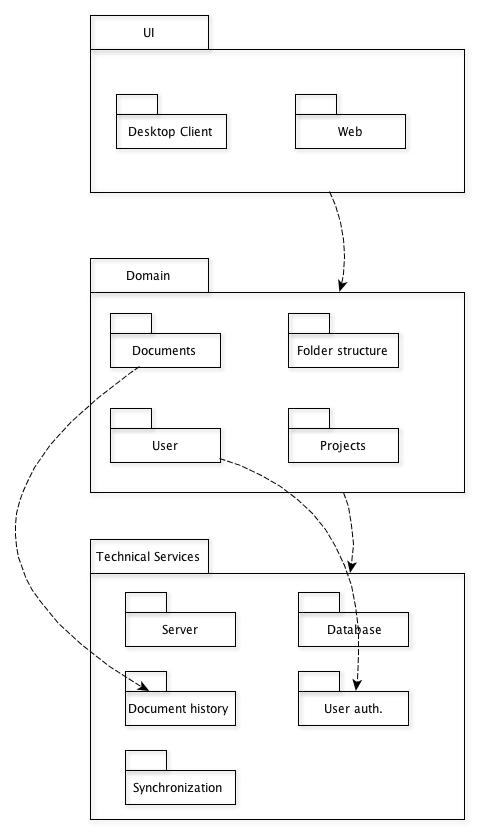
\includegraphics[width=300px]{images/LogicalArchitecture.jpg}
    	\caption{Logical Architecture}
	\end{figure}

\newpage
\section{Revision Table}
\begin{table}[ht]
\caption{Revision Table}
\begin{center}
\begin{tabular}{c|c|c}
\hline 
Revision & Changes & Section \\ \hline 
21-11-12 & Created Vision & 1 \\ 
21-11-12 & Created Use cases & 2 \\
21-11-12 & Created Glossary & 3 \\
21-11-12 & Created Supplementary Specifications & 4 \\ 
21-11-12 & Created Domain Model diagram & 5 \\
21-11-12 & Created Logical Architecture diagram & 6 \\
\hline 
\end{tabular} 
\end{center}
\end{table}
	
\end{document}